% Graphical model (single column): the accelerating accumulator with its
% three measurement models -- vocabulary (CDI items), input (recordings),
% processing (looking-while-listening trials) -- and the structural links
% that carry input and processing into efficiency (xi) and acceleration
% (kappa). Notation follows the manuscript's Model section:
%   xi_i    = mu_xi    + d_i        + beta_w  w_i + alpha_i
%   kappa_i = mu_kappa + beta_d d_i + beta'_w w_i + zeta_i
%   theta_i(t) = xi_i + kappa_i log(t / a_0)
%   y_ijt ~ Bernoulli(logit^{-1}(theta_i(t) + log H - delta_j))   (CDI item j)
%   r_iv  ~ N(mu_{r,s} + d_i, sigma_m[instrument])                 (recording v)
%   q_in  ~ N(tau_s + w_i + psi log(t_n / a_0), sigma_q)           (LWL trial n)
% Shaded = observed; circles = latent; rounded boxes = deterministic;
% dashed circle = fixed input; small squares = study / instrument constants.
% Compile: pdflatex fig_graphical_model.tex  (render_all.sh does this)
\documentclass[border=6pt]{standalone}
\usepackage{tikz}
\usepackage{amsmath}
\usetikzlibrary{positioning,calc,fit,arrows.meta,backgrounds}
\tikzset{
  lat/.style ={circle, draw=black, fill=white,   minimum size=0.9cm, inner sep=1pt},
  res/.style ={circle, draw=black!55, fill=white, minimum size=0.6cm, inner sep=0pt, font=\small},
  det/.style ={rectangle, rounded corners=3pt, draw=black, fill=blue!7, minimum height=0.8cm, inner sep=4pt},
  obs/.style ={circle, draw=black, fill=black!14, minimum size=0.9cm, inner sep=1pt},
  inp/.style ={circle, draw=black!55, dashed, fill=white, minimum size=0.62cm, inner sep=1pt, font=\small},
  stu/.style ={rectangle, draw=black!55, fill=white, minimum size=0.6cm, inner sep=2pt, font=\small},
  pl/.style  ={draw=black!50, rounded corners=5pt, inner sep=8pt},
  pll/.style ={font=\footnotesize\itshape, black!55},
  e/.style   ={-{Latex[length=1.8mm]}, draw=black!75},
  el/.style  ={font=\small, inner sep=1.2pt, fill=white},
  hdr/.style ={font=\footnotesize\bfseries, black!60},
}
\begin{document}
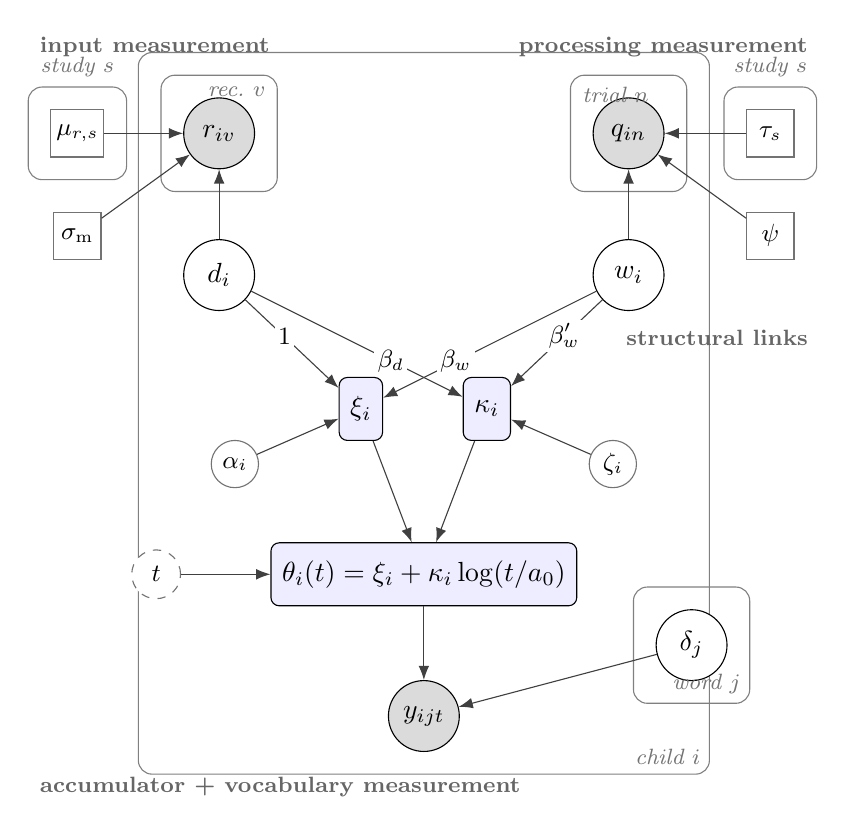
\begin{tikzpicture}
%% ---------- measurement models (top) ----------
% input: recordings r_{iv} read the child's input deviation d_i
\node[obs] (r)   at (-0.6, 5.2) {$r_{iv}$};
\node[lat] (d)   at (-0.6, 3.4) {$d_i$};
\node[stu] (mur) at (-2.4, 5.2) {$\mu_{r,s}$};
\node[stu] (sme) at (-2.4, 3.9) {$\sigma_{\mathrm{m}}$};
\draw[e] (d) -- (r);  \draw[e] (mur) -- (r); \draw[e] (sme) -- (r);
% processing: LWL trials q_{in} read the child's processing deviation w_i
\node[obs] (q)   at (4.6, 5.2) {$q_{in}$};
\node[lat] (w)   at (4.6, 3.4) {$w_i$};
\node[stu] (tau) at (6.4, 5.2) {$\tau_s$};
\node[stu] (psi) at (6.4, 3.9) {$\psi$};
\draw[e] (w) -- (q);  \draw[e] (tau) -- (q); \draw[e] (psi) -- (q);
%% ---------- structural links: traits ----------
\node[det] (xi) at (1.2, 1.7) {$\xi_i$};
\node[det] (ka) at (2.8, 1.7) {$\kappa_i$};
\node[res] (al) at (-0.4, 1.0) {$\alpha_i$};
\node[res] (ze) at (4.4, 1.0) {$\zeta_i$};
\draw[e] (d) -- (xi) node[el, pos=.42] {$1$};
\draw[e] (d) -- (ka) node[el, pos=.66] {$\beta_d$};
\draw[e] (w) -- (xi) node[el, pos=.66] {$\beta_w$};
\draw[e] (w) -- (ka) node[el, pos=.42] {$\beta'_w$};
\draw[e] (al) -- (xi); \draw[e] (ze) -- (ka);
%% ---------- accumulator core (bottom) ----------
\node[det] (th) at (2.0, -0.4) {$\theta_i(t)=\xi_i+\kappa_i\log(t/a_0)$};
\node[inp] (t)  at (-1.4, -0.4) {$t$};
\node[obs] (y)  at (2.0, -2.2) {$y_{ijt}$};
\node[lat] (de) at (5.4, -1.3) {$\delta_j$};
\draw[e] (xi) -- (th); \draw[e] (ka) -- (th); \draw[e] (t) -- (th);
\draw[e] (th) -- (y);  \draw[e] (de) -- (y);
%% ---------- plates ----------
\begin{scope}[on background layer]
\node[pl, fit=(r)]  (recpl) {};
\node[pl, fit=(q)]  (lwlpl) {};
\node[pl, fit=(recpl)(lwlpl)(d)(w)(xi)(ka)(al)(ze)(th)(y)] (childpl) {};
\node[pl, fit=(de)] (wordpl) {};
\node[pl, fit=(mur)] (stuA) {};
\node[pl, fit=(tau)] (stuB) {};
\end{scope}
% plate labels placed away from the arrows
\node[pll, anchor=north east] at ([xshift=-1pt,yshift=-1pt]recpl.north east) {rec.\ $v$};
\node[pll, anchor=north west] at ([xshift=1pt,yshift=-1pt]lwlpl.north west) {trial $n$};
\node[pll, anchor=south east] at (childpl.south east) {child $i$};
\node[pll, anchor=south east] at (wordpl.south east) {word $j$};
\node[pll, anchor=south] at (stuA.north) {study $s$};
\node[pll, anchor=south] at (stuB.north) {study $s$};
% section headers
\node[hdr, anchor=west] at (-3.0, 6.3) {input measurement};
\node[hdr, anchor=east] at (7.0, 6.3) {processing measurement};
\node[hdr, anchor=east] at (7.0, 2.6) {structural links};
\node[hdr, anchor=west] at (-3.0, -3.1) {accumulator + vocabulary measurement};
\end{tikzpicture}
\end{document}
